\graphicspath{ {Figures/Pileup/} {Figures/Main/} {Figures/ResidualsFFT/} }

\chapter{Analysis Results}

\section{Pre-corrected and corrected energy and time spectra}

\begin{figure}[h]
	\centering
	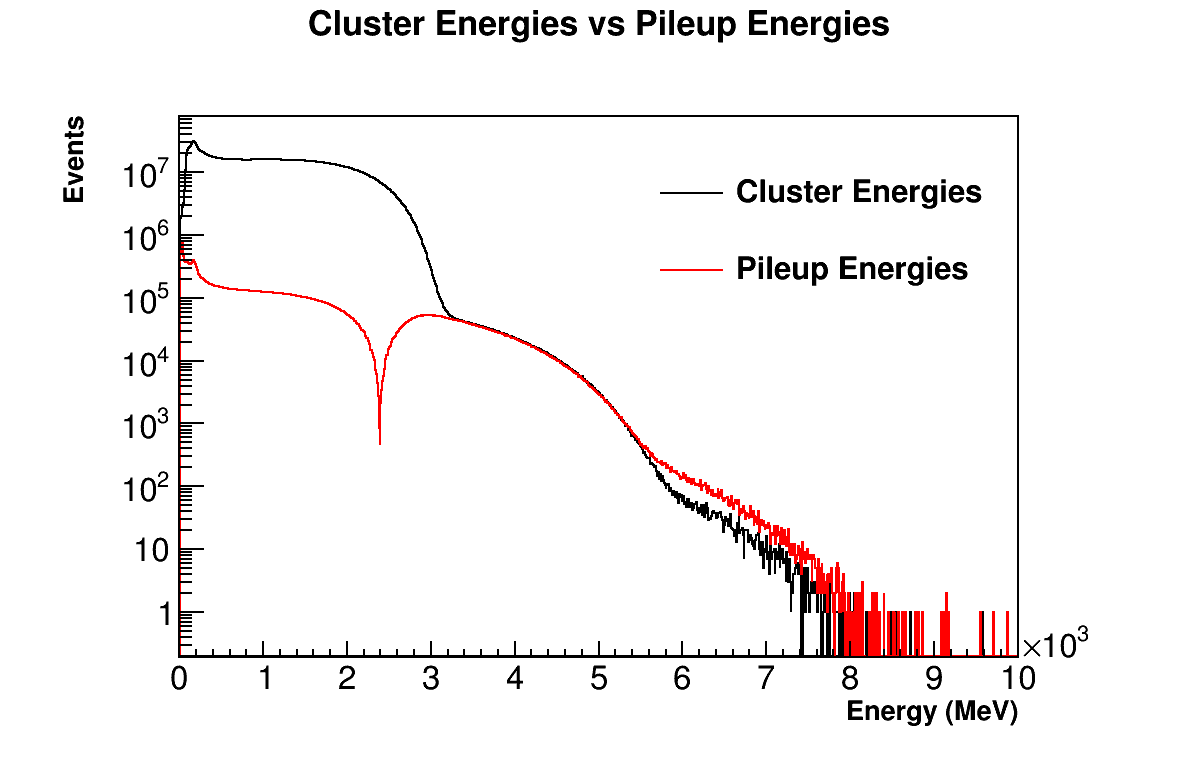
\includegraphics[width=\textwidth]{ClusterEnergiesVsPileupEnergies}
    \caption[ClusterEnergiesVsPileupEnergies]{Cluster energies in black are plotted vs pileup energies in red, for all calorimeters added together. At energies below about 2.4 GeV the pileup spectrum goes negative. In this plot the absolute value of the pileup energies is plotted, and a spike at about 2.4 GeV can be seen as a consequence of this. Due to the triplets and contamination in the pileup spectrum, the red and black curves can be seen to diverge at high energies.}    
    \label{fig:ClusterEnergiesVsPileupEnergies}
\end{figure}

\begin{figure}[]
\centering
    \begin{subfigure}[]{0.8\textwidth}
	    \centering
		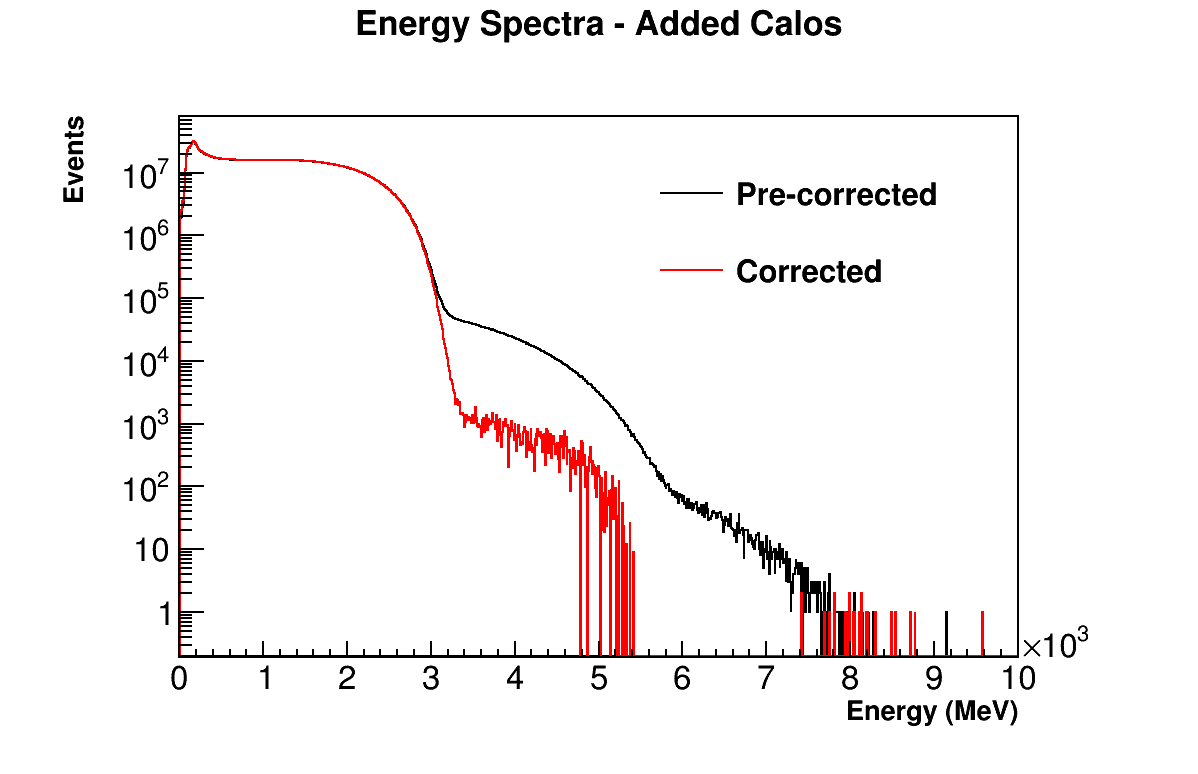
\includegraphics[width=\textwidth]{AddedEnergies}
	    \caption{Log scale - the corrected energy spectrum goes negative around 5 GeV.}
    \end{subfigure}% %you need this % here to add spacing between subfigures
    \vspace{1cm}
    \begin{subfigure}[]{0.8\textwidth}
	    \centering
		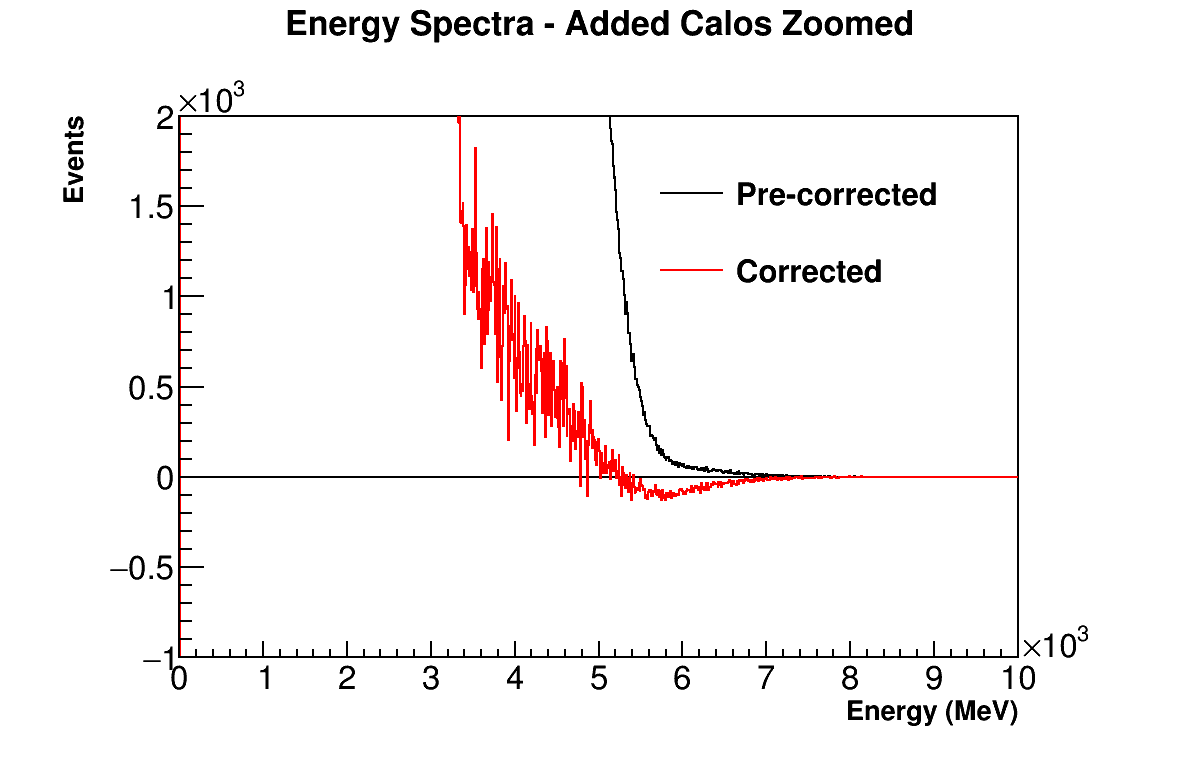
\includegraphics[width=\textwidth]{AddedEnergiesZoomed}
	    \caption{Linear scale - zoomed in to show the shape.}
    \end{subfigure}
\caption[AddedEnergies]{Plots for the pre-corrected and corrected energy spectra are shown, all calorimeters added together. Because the triplets and contamination are not accounted for, the corrected energy spectrum does not lie exacltly along zero.}
\label{fig:AddedEnergies}
\end{figure}

\begin{figure}[]
	\centering
	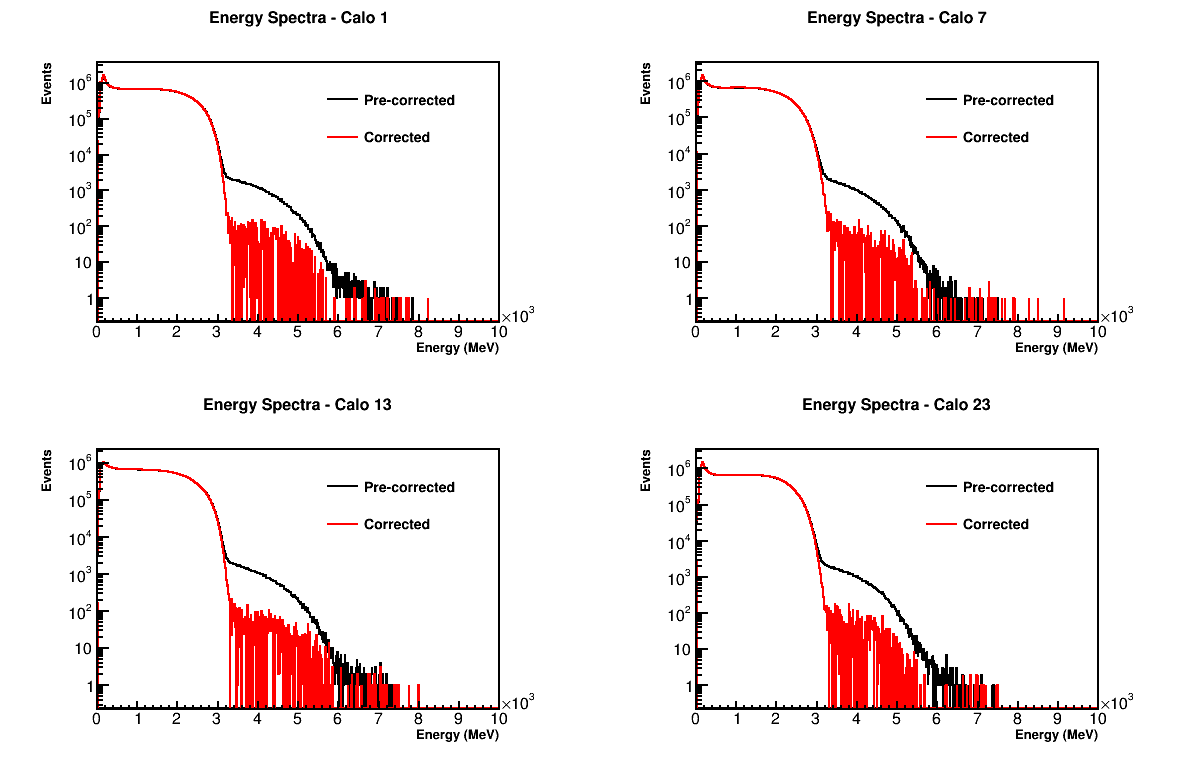
\includegraphics[width=\textwidth]{CaloEnergies}
    \caption[CaloEnergies]{Pre-corrected and corrected energy spectra for calorimeters 1, 7, 13, and 23 plotted on a log scale.}    
    \label{fig:CaloEnergies}
\end{figure}

\begin{figure}[]
	\centering
	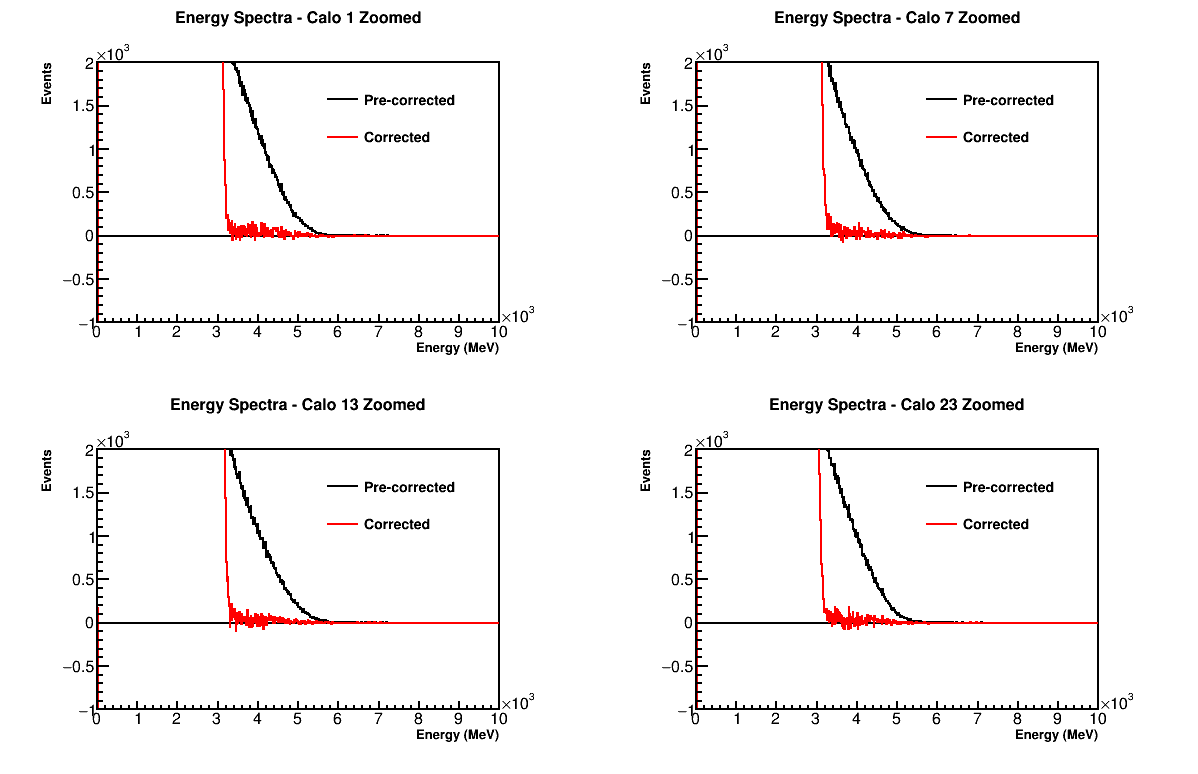
\includegraphics[width=\textwidth]{CaloEnergiesZoomed}
    \caption[CaloEnergiesZoomed]{Pre-corrected and corrected energy spectra for calorimeters 1, 7, 13, and 23 plotted on a linear scale and zoomed in.}    
    \label{fig:CaloEnergiesZoomed}
\end{figure}



\section{6 Parameter Ratio Fit}

\begin{figure}[H]
	\centering
	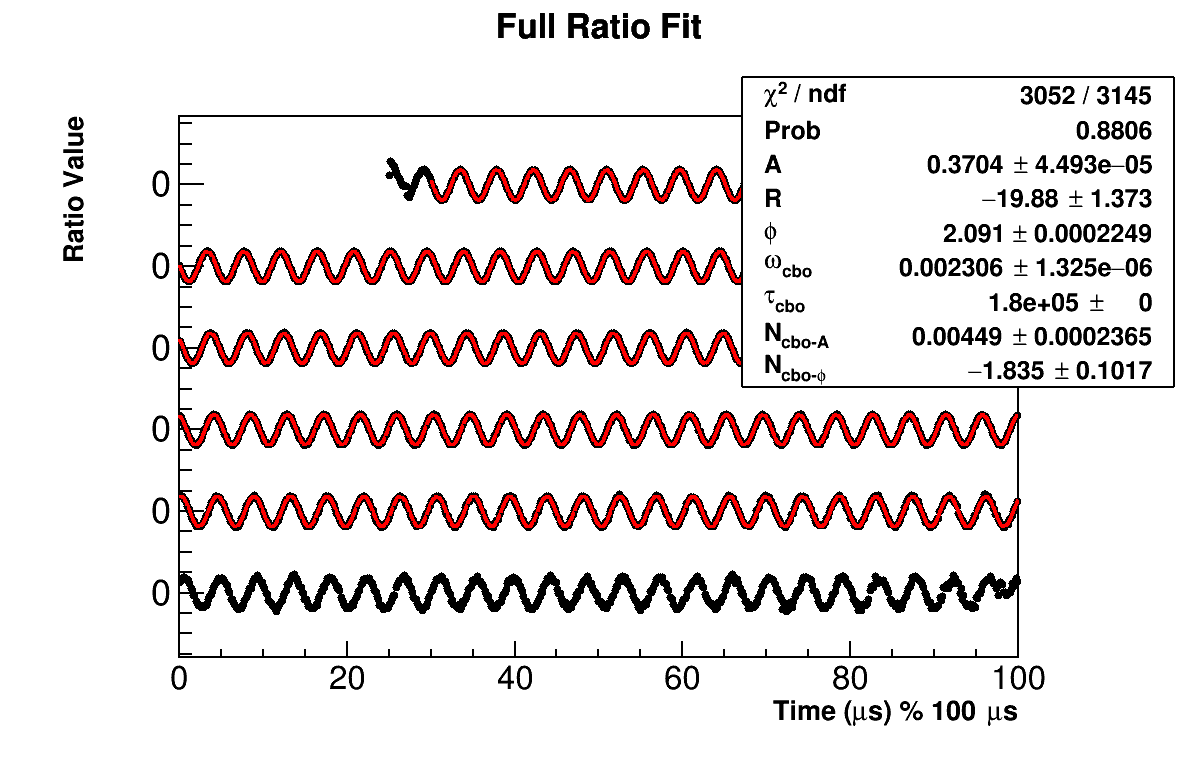
\includegraphics[width=\textwidth]{ratioCBO_moduloPlot}
    \caption[ratioCBO_moduloPlot]{Final fit result for the 60 hour dataset. The fit includes 6 free parameters and one fixed. The x axis is in units of $\mu$s modulo 100 $\mu$s, with successive portions of the data points and fit shifted downwards on the plot. The parameter values in the stats box for the CBO frequency and lifetime are in units of ns. R is blinded locally. The fit ranges from 30 $\mu$s to 500 $\mu$s.}
    \label{fig:ratioCBO_moduloPlot}
\end{figure}



\section{Residual and FFT}

\begin{figure}[H]
\centering
    \begin{subfigure}[]{0.45\textwidth}
	    \centering
		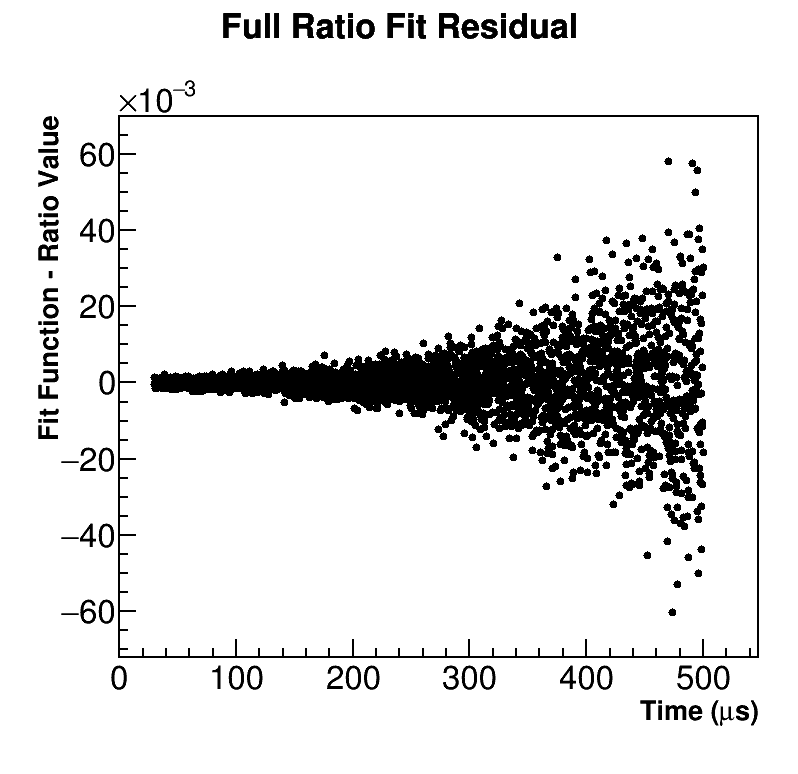
\includegraphics[width=\textwidth]{fitResidual}
	    \caption{Fit residuals.}
    \end{subfigure}
    \begin{subfigure}[]{0.45\textwidth}
	    \centering
		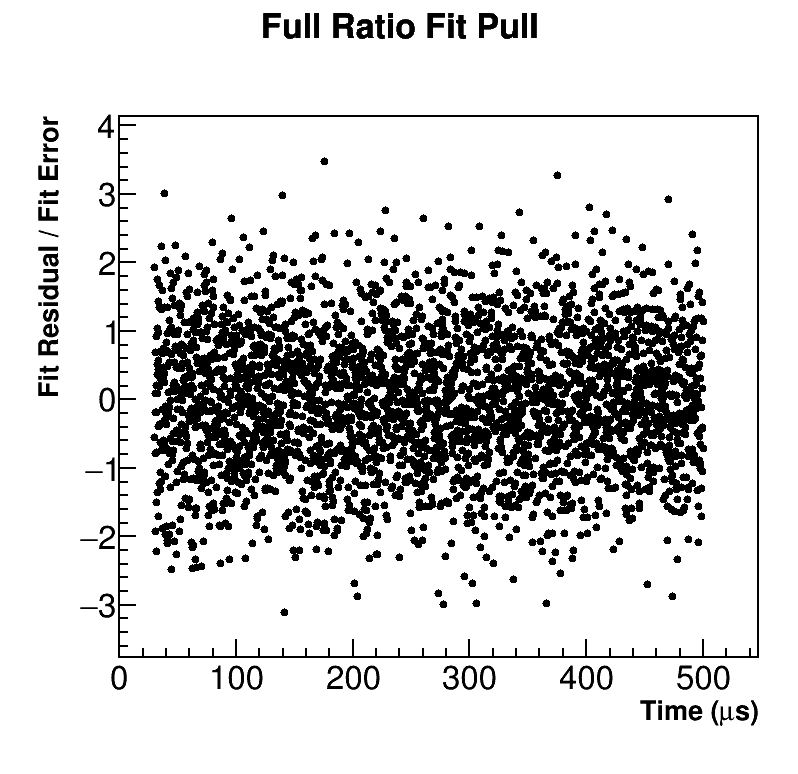
\includegraphics[width=\textwidth]{fitPull}
	    \caption{Fit pulls.}
    \end{subfigure}% %you need this % here to add spacing between subfigures
    \vspace{4mm}
    \begin{subfigure}[]{0.7\textwidth}
	    \centering
		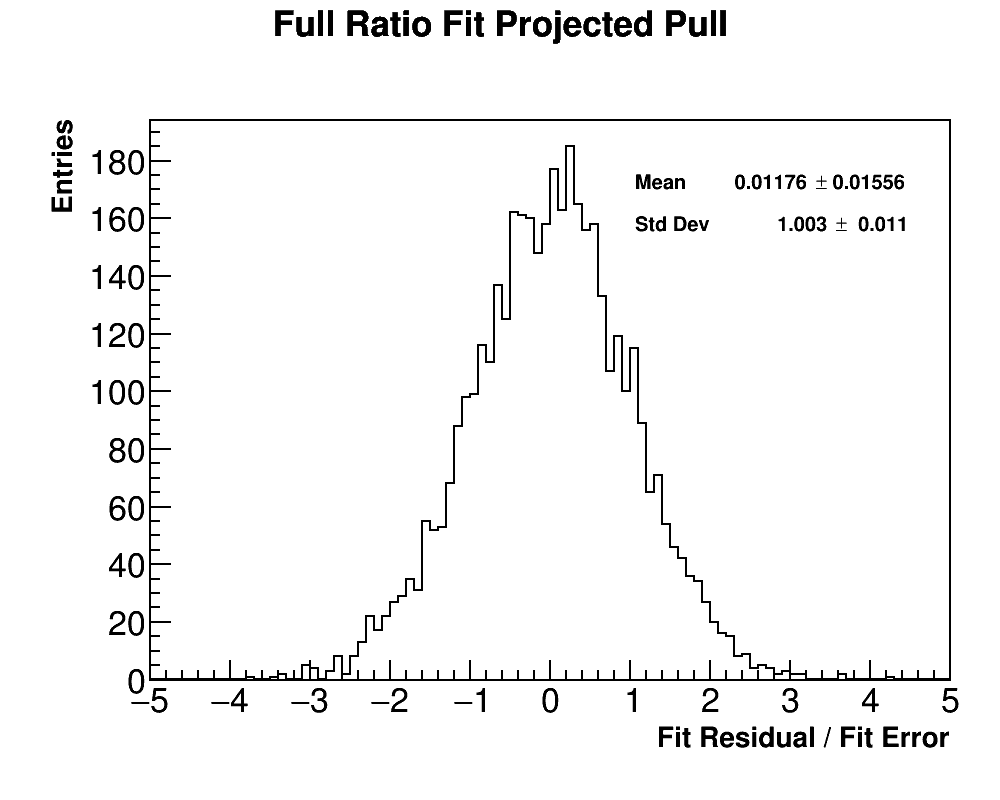
\includegraphics[width=\textwidth]{fitPull_projected}
	    \caption{Fit pulls projected onto the y axis. Note the Gaussian shape centered around 0 with unit width.}
    \end{subfigure}
\caption[fitResidual]{Residuals and pulls for the full ratio fit.}
\label{fig:fitResidual}
\end{figure}






\section{Start time scans}


\section{Results vs calorimeter}



\section{Correlation matrix for fit parameters}



